\chapter{Method}
\label{chap:method}

We start of at the same spot we left of after the thesis. Before we go on to explain what's been done this semester, lets recap. 

We started off by just getting a drive with lots of \acrshort{das} data, and a script from \acrfull{asn} which set up us perfectly. We chose to rewrite python code to a language similar to that of MAtlab and Python. We landed on Julia, and with its broad ecosytstem it has support for all kinds of development we'd ever need. \\

We first wrote a 1:1 copy of the script, and then parallellized parts of the code until we had a version that could handle large amounts of data in parallel. We also wrote methods for being able to run a window over and 


\section{Overview}

The \acrshort{api} that's being created is called \texttt{Judas} (Julia and DAS) and is split in 3 modules as well as a seperate Utils file as shown in \ref{fig:ccuda}

\begin{figure}[h]
    \centering
    \includegraphics{figures/overview.png}
    \caption{Overview over our package Judas}
    \label{fig:judasoverview}
\end{figure}


\section{DAS.jl}

The DAS folder has not changed much substantially. The main difference from before is how we now instead of writing matrix data to one large binary file, data is split into multiple files, and only read when needed.

\section{SignalProcessing.jl}

After data has been read and processed, it's ready to be processed by signal processing functions 

\section{AI.jl}

The main aspects of this code lies within the module \texttt{AI.jl}. 




\subsection{JudasNET}

\texttt{JudasNET} is the architecture of choice for interpreting data

\begin{figure}{h}
    \centering
    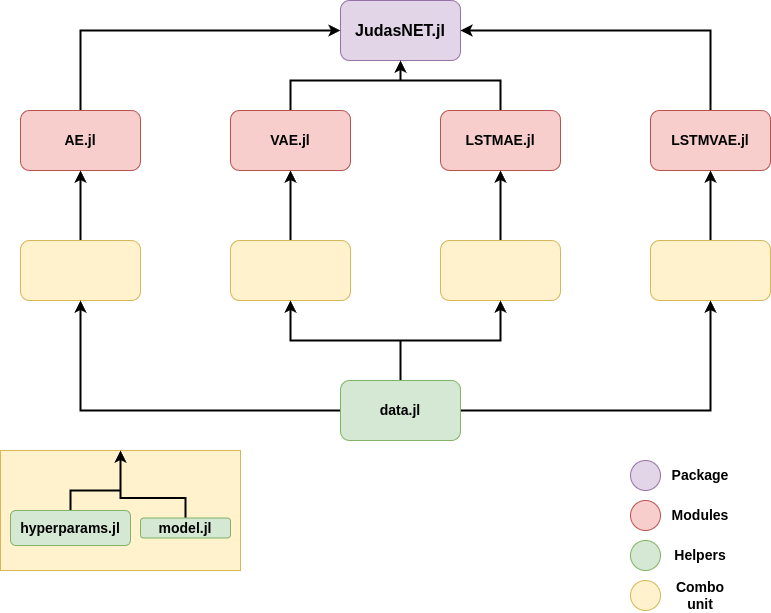
\includegraphics{figures/judasnet.png}
    \caption{Flowchart over JudasNET}
    \label{fig:judasnet}
\end{figure}